\section{Introduction}

%%%%%%%%%%%%%%%%%%%%%%%%%%%%%%%%%%%%%%%%%%%%%%%%%%%%%%%%%%%%%%%%%%%%%%%%%%%%%%%
\begin{frame}{A very casual motivation}


\begin{center}
\Large
I want to host \textbf{resilient web services} with \textbf{acceptable performance} on commodity hardware behind \textbf{household networks}.
\end{center}
\vfill

\begin{block}{Keywords}
\begin{columns}
\column{.5\columnwidth}
	\begin{itemize}
		\item Decentralised networks
		\item Edge computing
	\end{itemize}
\column{.5\columnwidth}
	\begin{itemize}
		\item Distributed storage
		\item Privacy
	\end{itemize}
\end{columns}
\end{block}

\end{frame}

%%%%%%%%%%%%%%%%%%%%%%%%%%%%%%%%%%%%%%%%%%%%%%%%%%%%%%%%%%%%%%%%%%%%%%%%%%%%%%%
\begin{frame}{Context}

\textbf{Resilience}: Ability to recover quickly from failures and changes.
\vspace{1ex}

Only achievable through distribution of the hosted applications across several physical locations.
\vfill


\begin{block}{Application = \textbf{computations} on \textbf{data}}
\begin{itemize}
	\item \textbf{Computation}: Stateless; easy to distribute \& orchestrate.
	% where it is performed does not matter as long as the application's state is accessible R/W
	%Computation units are "easy" to distribute and orchestrate.

	\item \textbf{Data}: Stateful; hard to distribute \& full of trade-offs.
\end{itemize}
\end{block}

\end{frame}


%%%%%%%%%%%%%%%%%%%%%%%%%%%%%%%%%%%%%%%%%%%%%%%%%%%%%%%%%%%%%%%%%%%%%%%%%%%%%%%
\begin{frame}{Concurrent writes example}{How to lose vaccines}

\centering

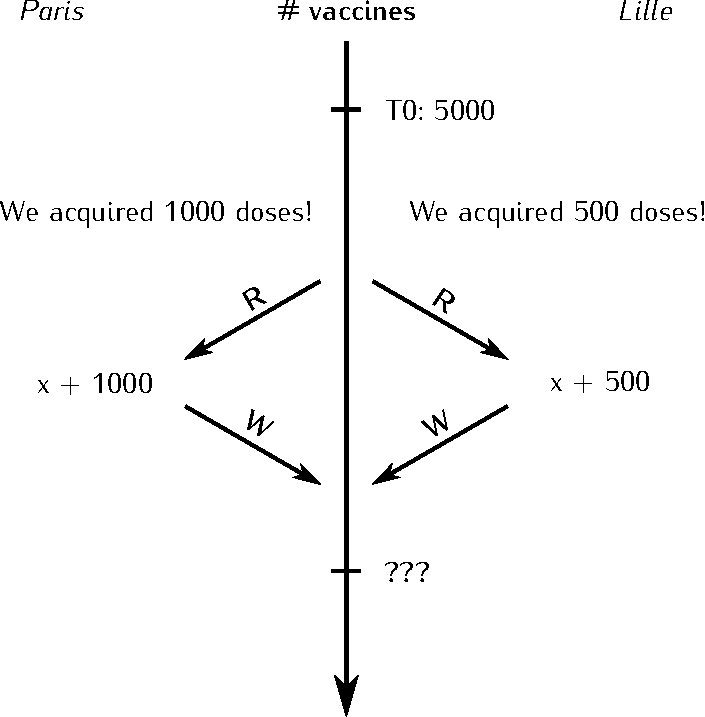
\includegraphics[width=.5\columnwidth]{figures/conflict_problem.pdf}
\end{frame}

%%%%%%%%%%%%%%%%%%%%%%%%%%%%%%%%%%%%%%%%%%%%%%%%%%%%%%%%%%%%%%%%%%%%%%%%%%%%%%%
\begin{frame}{The problem}

% \textbf{Path dependency}: existing data stores are built for data centres.

% $\implies$ They assume good inter-node connectivity.
% \vfill

\begin{center}
\Large
Can we design an available data store tailored for adverse network conditions?
\end{center}
	
\end{frame}

%%%%%%%%%%%%%%%%%%%%%%%%%%%%%%%%%%%%%%%%%%%%%%%%%%%%%%%%%%%%%%%%%%%%%%%%%%%%%%%
%%%%%%%%%%%%%%%%%%%%%%%%%%%%%%%%%%%%%%%%%%%%%%%%%%%%%%%%%%%%%%%%%%%%%%%%%%%%%%%
% Maybe more framing of the context. What kind of data storage? Object vs Block vs what?
% \begin{frame}{``Stateless'', ``serverless'', and the elephant in the room}

% It seems easy to deploy \& administer web services nowadays ...

% Because the inherent complexity is shadowed by proprietary ``cloud'' solutions.

% The IT crowd can gloss over ``statelessness'' \emph{ad nauseam} ...

% But storing \emph{state} remains an open research problem.

% Data storage is either:

% \begin{itemize}
% 	\item A single point of failure;
% 	\item Delegated to proprietary solutions;
% 	\item Pain.
% \end{itemize}

% Today, we will review networked storage's history, and discuss open research questions.

% \end{frame}